% !TEX root = ../main.tex
\begin{figure}[t]
\centering
\iflatexml
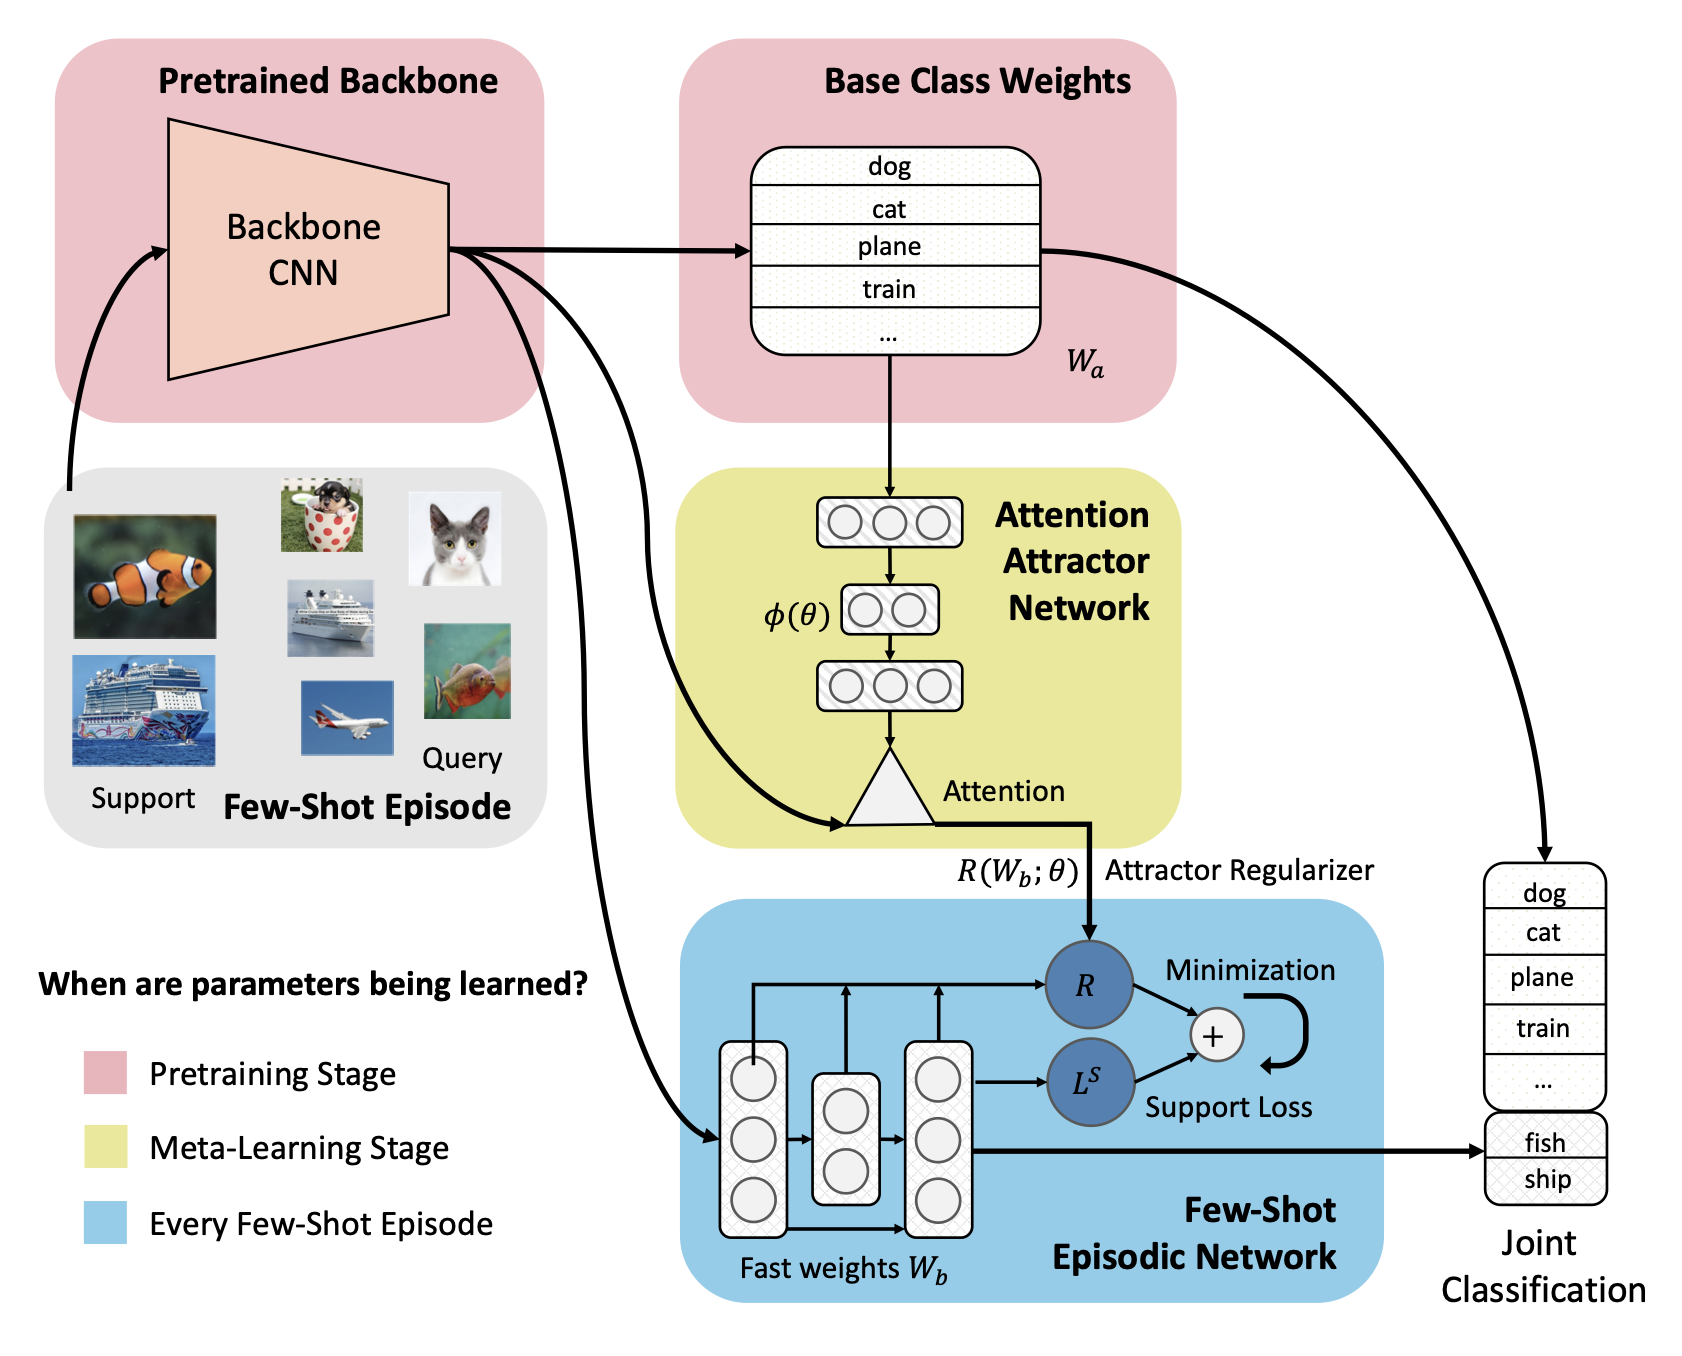
\includegraphics[width=6\textwidth]{figures/mainfig.png}
\else
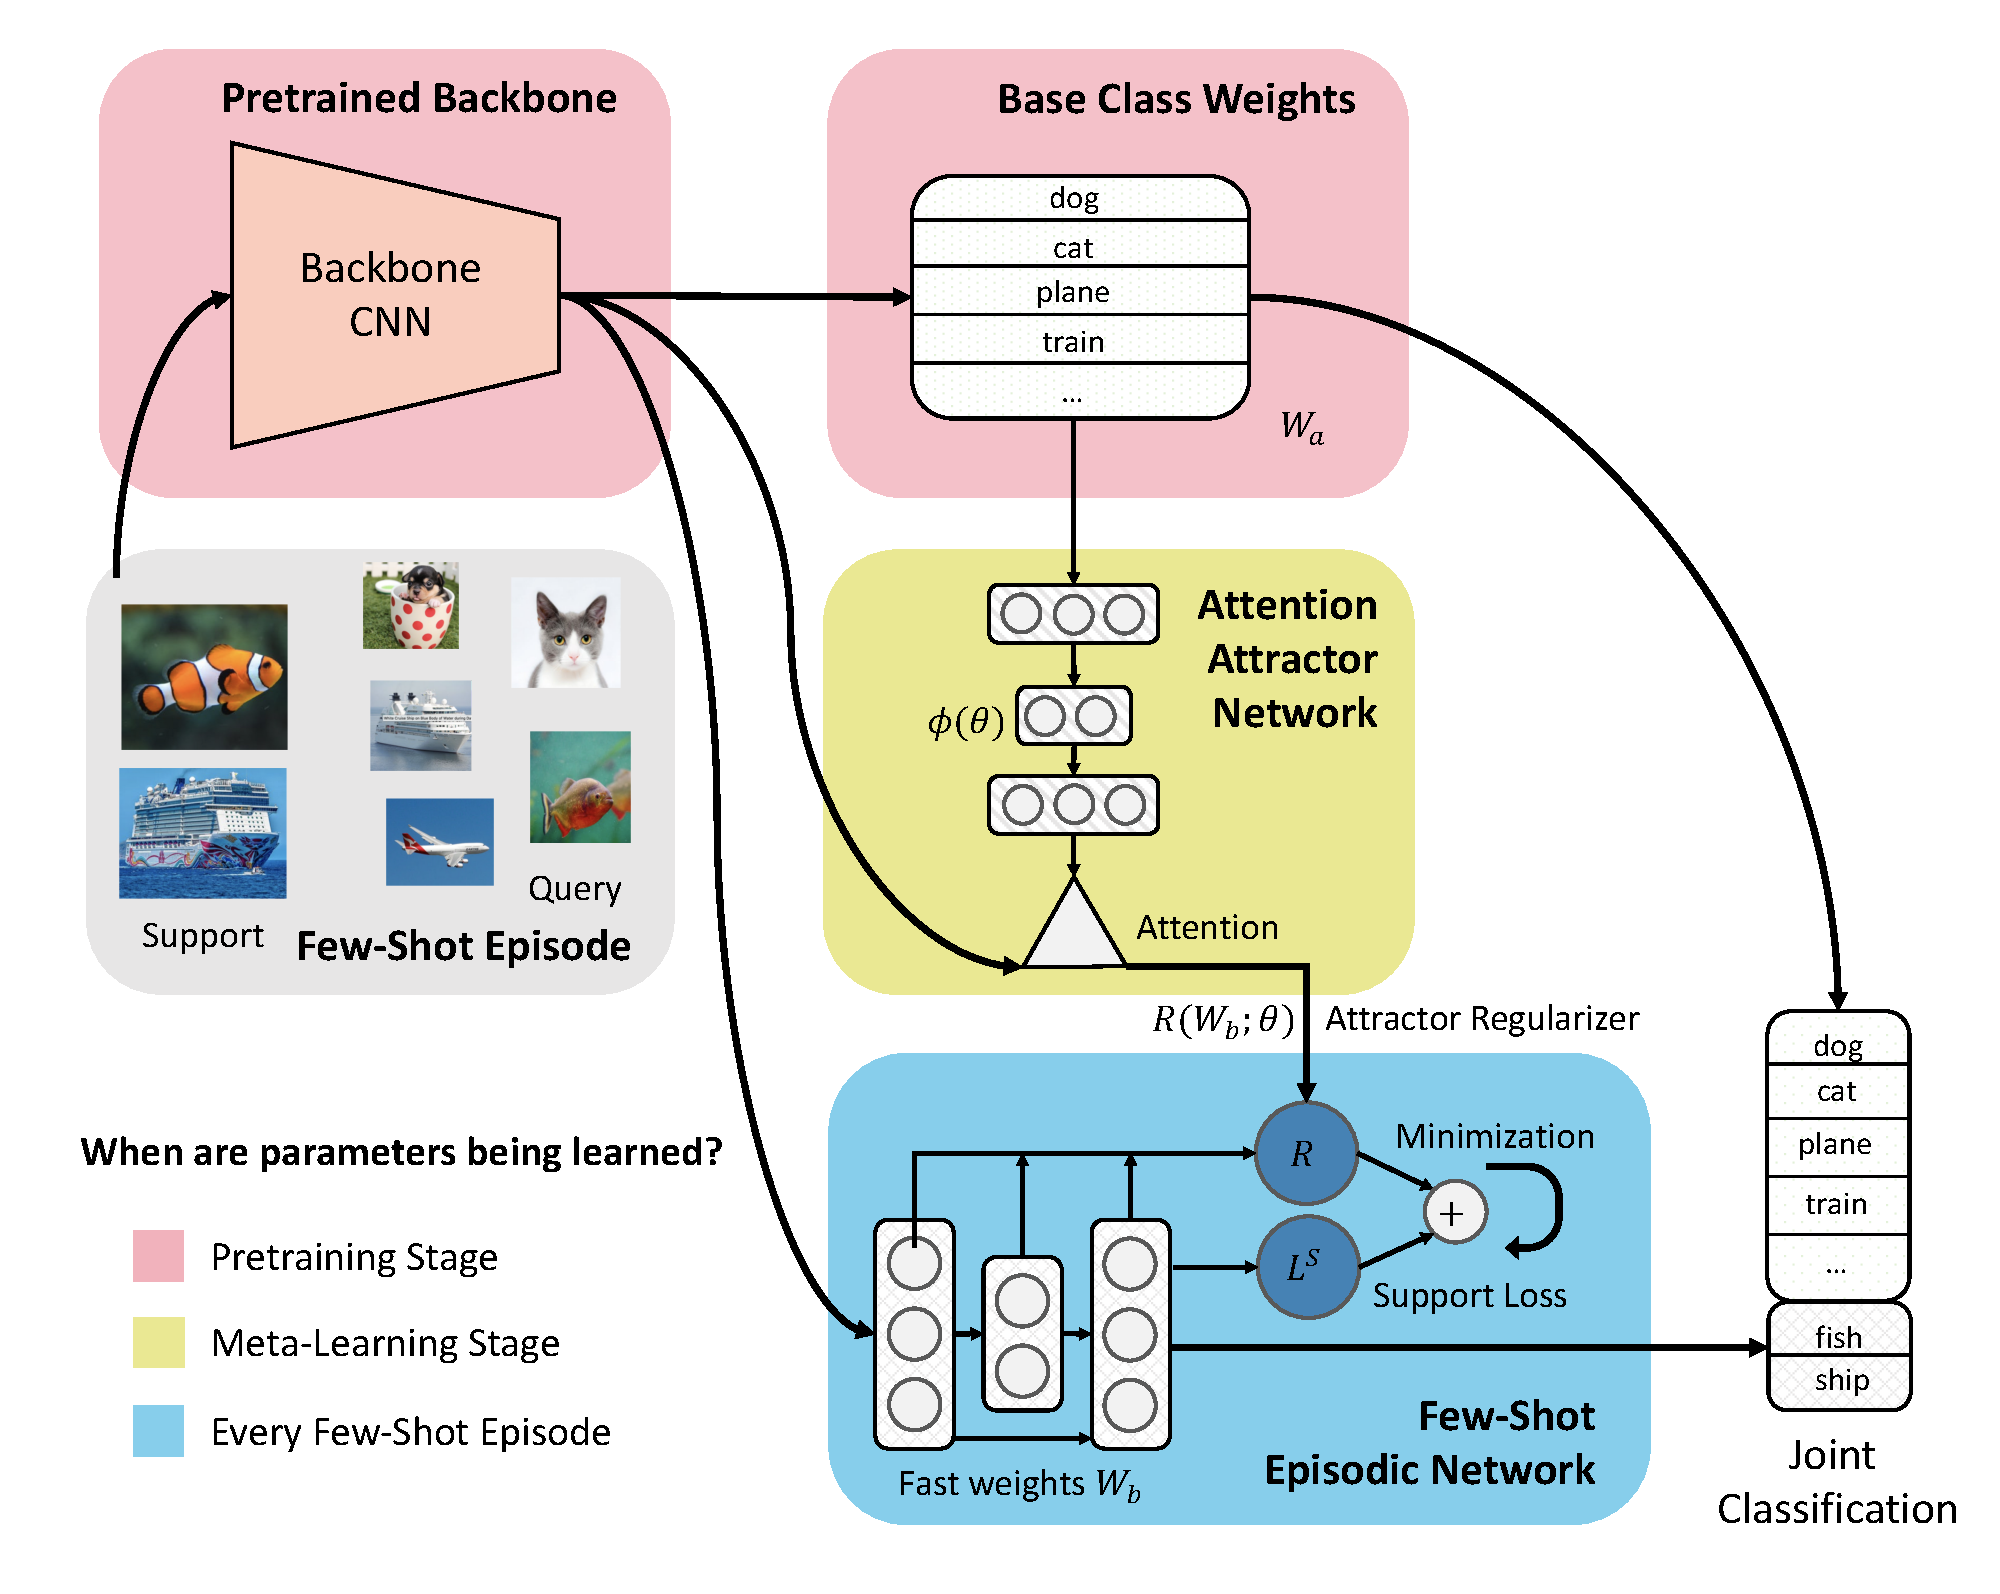
\includegraphics[width=0.7\textwidth,trim={1cm 0 0 0.7cm},clip]{figures/attractor_v4.pdf}
\fi
\caption{Our proposed attention attractor network for incremental few-shot learning.
During pretraining we learn the base class weights $W_a$ and the feature extractor CNN backbone. In
the meta-learning stage, a few-shot episode is presented. The support set only contains novel
classes, whereas the query set contains both base and novel classes. We learn an episodic classifier
network through an iterative solver, to minimize cross entropy plus an additional regularization
term predicted by the attention attractor network by attending to the base classes. The attention
attractor network is meta-learned to minimize the expected query loss. During testing an episodic
classifier is learned in the same way.}
\label{fig:model}
\end{figure}